\documentclass[12pt, a4paper, oneside]{ctexart}
\usepackage{amsmath,extarrows, amsthm, amssymb, bm, graphicx,listings, hyperref, geometry, mathrsfs,color, tikz}
\usetikzlibrary{shapes,arrows,positioning}

%% cpp code setting
\usepackage{xcolor}
\lstset{
    language=C++,
    basicstyle=\footnotesize\ttfamily, 
    numbers=left, 
    numberstyle=\tiny\color{gray}, 
    stepnumber=1, 
    numbersep=5pt, 
    backgroundcolor=\color{white}, 
    showspaces=false, 
    showstringspaces=false, 
    showtabs=false, 
    tabsize=2, 
    captionpos=b, 
    breaklines=true, 
    breakatwhitespace=false, 
    escapeinside={\%*}{*},
    keywordstyle=\color{blue},
    commentstyle=\color{ForestGreen},
    stringstyle=\color{purple},
    morecomment=[l][\color{magenta}]{\#}
}

\title{\huge\textbf{DS项目作业2}}
\author{罗俊勋}
\date{\today}
\linespread{2}%行间距
\geometry{left=2cm,right=2cm,top=2cm,bottom=2cm}%设置页面
\CTEXsetup[format={\Large\bfseries}]{section}%section左对齐

%定义环境
\newenvironment{Def}[1][def-name]{\par\noindent{\textit{(#1):}\small}}{\\\par}
\newenvironment{theorem}[1][Theorem-name]{\par\noindent \textbf{Theorem #1:}\textit}{\\\par}
\newenvironment{corollary}[1][corollary-name]{\par\noindent \textbf{Corollary #1:}\textit}{\\\par\vspace*{15pt}}
\newenvironment{lemma}[1][lemma-name]{\par\noindent \textbf{Lemma #1:}\textbf}{\\\par}
\renewenvironment{proof}{\par\noindent{\textit{Proof:}\small}}{\\\par}
\newenvironment{example}[1][example-name]{\par{\textbf{Example:}}}{\\\par}
\newenvironment{say}{\center{\textit{summary:}}}{\\\par}
\newenvironment{note}[1][note-name]{\par\textit{#1:}}{\\\par}
\newcommand{\qie}{\enspace\&\enspace}


\begin{document}
\maketitle
\section*{项目说明}
我们课本提供的 code 当中(可以在群文件中下载), 已经提供了 BinarySearchTree.h, AvlTree.h, RedBlackTree.h 和 SplayTree.h, 分别实现了对应的功能. 由于是教学代码, 每一个头文件都是独立的. 现在, 请根据它们各自的用途, 整理它们的逻辑关系, 重构全部代码, 并用继承关系予以表达. 要求:

1. 尽量使用已有代码, 并且不要丢失任何功能;

2. 用继承关系体现它们彼此之间的逻辑关系, 可以根据需要增加虚类, 改变成员变量或成员函数开放属性;

3. 至少增加一个基础虚类: BinaryTree, 作为最顶级的基类, 用以规范全部二叉树的基本操作;

4. 请同步考虑各种 Node 之间的关系和结构;

$5^*$. 鼓励使用多态, 或提供多态接口;

6. 将全部代码整合成一个 BinaryTree.h 文件, 并辅以必要的注释;

7. 提供文件 report.pdf 说明你的设计思路, 鼓励使用 latex 和 uml (不知道的同学可以忽略) ;

8. 参考 code 中的 TestBinarySearchTree.cpp, TestAvITree.cpp, TestRedBlackTree.cpp 和 TestSplayTree.cpp 等文件, 构建一个 TestTree.cpp 文件, 测试你的全部代码.

9. 本项目作业在期末考前终止. 过时不补交.

\section*{设计思路}
- BinaryTree : 这是最基础的二叉树类,定义了二叉树的基本操作。

- BinarySearchTree:这个类继承自 BinaryTree,实现了二叉搜索树的特性。

- AvITree:这个类继承自 BinarySearchTree,实现了AVL树的特性。

- RedBlackTree:这个类也继承自 BinarySearchTree,实现了红黑树的特性。

- SplayTree:这个类同样继承自 BinarySearchTree,实现了伸展树的特性。

代码示例如下
\begin{lstlisting}[caption={}]
    template <typename Comparable>
    class BinaryTree{};
    
    template <typename Comparable>
    class BinarySearchTree: public BinaryTree<Comparable>{};
    
    template <typename Comparable>
    class AvlTree: public BinarySearchTree<Comparable>{};
    
    template <typename Comparable>
    class RedBlackTree: public BinarySearchTree<Comparable>{};
    
    template <typename Comparable>
    class SplayTree: public BinarySearchTree<Comparable>{};
\end{lstlisting}

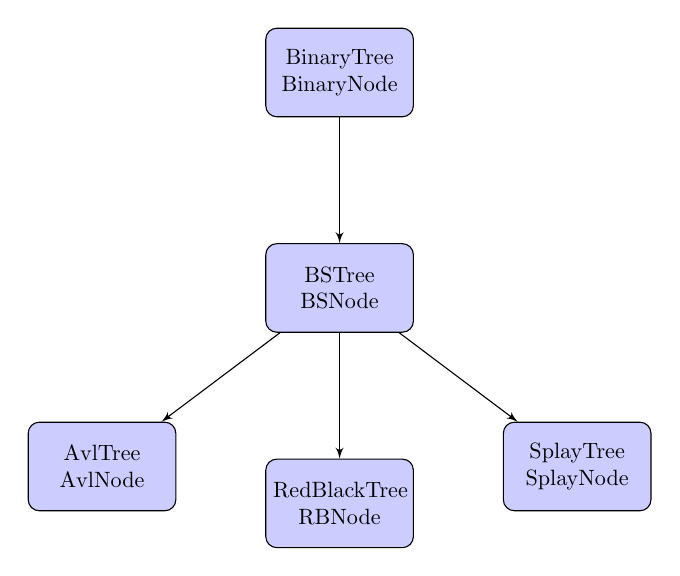
\begin{tikzpicture}[
    node distance=2cm,
    class/.style={rectangle, draw=black, fill=blue!20, text width=6em, text centered, rounded corners, minimum height=4em},
    line/.style={draw, -latex'},
    scale=0.8, every node/.style={transform shape}
  ]
    \node [class] (binarytree) {BinaryTree\\BinaryNode};
    \node [class, below=of binarytree] (binarysearchtree) {BSTree\\BSNode};
    \node [class, below left=of binarysearchtree] (avltree) {AvlTree\\AvlNode};
    \node [class, below=of binarysearchtree] (redblacktree) {RedBlackTree\\RBNode};
    \node [class, below right=of binarysearchtree] (splaytree) {SplayTree\\SplayNode};
  
    \path [line] (binarytree) -- (binarysearchtree);
    \path [line] (binarysearchtree) -- (avltree);
    \path [line] (binarysearchtree) -- (redblacktree);
    \path [line] (binarysearchtree) -- (splaytree);
\end{tikzpicture}





\end{document}
